\documentclass[11pt]{article}

\usepackage[margin=1in]{geometry}
\usepackage{amsmath,amssymb,amsfonts}
\usepackage{graphicx}
\usepackage{booktabs}
\usepackage{hyperref}
\usepackage{caption}
\usepackage{subcaption}
\usepackage{microtype}

\graphicspath{{../../data/cfb/}}

\title{CFB: A Continual Forecasting Benchmark}
\author{Kevin Murphy \\\\ \texttt{murphyk@gmail.com}}
\date{\today \\ {\small (preliminary draft)}}

\begin{document}
\maketitle

\section{Setup}
\label{sec:setup}

CFB simulates an online prediction-market environment with delayed,
asynchronous feedback. Time advances in days $t \in \{t_0, t_0+1, \dots, t_{\max}\}$.
Each binary forecasting question $u$ in the universe $\mathcal{U}$ has
three immutable attributes: a forecast-due date $f_u$, a resolution date
$r_u \ge f_u$, and an outcome $o_u \in \{0, 1\}$.

On each day $t$ the agent interacts with the environment in three stages:

\paragraph{Observation.}
The fresh question batch and the resolution batch are
\begin{align}
  Q(t) &= \{ u \in \mathcal{U} : f_u = t \}, &
  R(t) &= \{ (u, o_u) : u \in \mathcal{U},\, r_u = t \}.
\end{align}

\paragraph{Action.}
The agent emits forecasts only for the freshly-asked questions:
\begin{equation}
  A(t) = \{ p_u \in [0, 1] : u \in Q(t) \},
  \qquad
  p_u \;=\; \pi\!\left(q_u, r_u \,\big|\, \mathcal{H}(<t)\right),
\end{equation}
where $\pi$ is the agent's policy and the information set is
\begin{equation}
  \mathcal{H}(<t) \;=\; \bigcup_{s < t} \big(Q(s), A(s), R(s)\big).
\end{equation}
That is, when forecasting on day $t$ the agent sees every prior question,
its own past forecasts, and every resolution that has \emph{already}
arrived. Today's resolutions $R(t)$ are revealed only after the action
$A(t)$ is committed.

\paragraph{Reward.}
The reward for an action $p_u$ taken on day $f_u$ is the Brier loss
$\ell_u = (p_u - o_u)^2$, and it is realized on day $r_u$ — typically days
to months later. Concretely, the resolution of $u$ enters the reward
stream on day $t = r_u$, so the per-day reward set is
\begin{equation}
  \mathcal{B}(t) = \{ \ell_u : u \in \mathcal{U},\, r_u = t \}.
\end{equation}
This is the asynchronous-reward structure: the action-to-reward delay
$r_u - f_u$ is question-specific and unbounded a priori.

\paragraph{Aggregate scores.}
After the run we report Brier and Brier index in two weightings. Let
$N = |\{u : r_u \le t_{\max}\}|$ be the number of resolved events, and
let $\mathcal{S}$ be the set of question sources. Define
\begin{align}
  \overline{B}_{\text{event}}
    &= \tfrac{1}{N}\textstyle\sum_{u : r_u \le t_{\max}} \ell_u, \\
  \overline{B}_{\text{source}}
    &= \tfrac{1}{|\mathcal{S}|}\textstyle\sum_{s \in \mathcal{S}}
       \tfrac{1}{N_s}\textstyle\sum_{u \in s : r_u \le t_{\max}} \ell_u.
\end{align}
The corresponding Brier indices are $\mathrm{BI} = 1 - 4\,\overline{B}$.

\section{Data}
\label{sec:data}

CFB is constructed from per-question JSON files downloaded by the
ForecastBench (FB) pipeline. Every question file carries a
\texttt{forecast\_due\_date} (the day the question was asked) and either
a single \texttt{resolution\_date} (markets) or a list of resolution dates
(dataset questions). Multi-resolution dataset questions are flattened so
each entry $u$ corresponds to exactly one $(f_u, r_u, o_u)$ triple.

Pool construction applies four filters in sequence:
\begin{enumerate}
  \item \emph{Window:} keep $u$ with $t_0 \le f_u$ and $r_u \le t_{\max}$.
        Censored entries ($r_u > t_{\max}$) are dropped because we will
        never observe their outcome before the simulation ends.
  \item \emph{Binary outcomes:} only $o_u \in \{0, 1\}$ survives; any
        fractional or null value is treated as unresolved and dropped.
  \item \emph{Dedupe-base:} the same underlying question may appear at
        multiple forecast dates with different reference values. We keep
        only the entry with the earliest $f_u$, retaining all of its
        resolution events.
  \item \emph{Source selection:} the canonical pool is
        \emph{markets-only} ---
        $\mathcal{S} = \{\text{polymarket}, \text{manifold},
                         \text{metaculus}, \text{infer}\}$. The
        \texttt{--use-data-and-market} flag re-includes the dataset
        sources (\texttt{acled}, \texttt{dbnomics}, \texttt{fred},
        \texttt{wikipedia}, \texttt{yfinance}) for stretch experiments.
\end{enumerate}

For the canonical CFB run we use $t_0 = $ 2025-10-26 (after the knowledge
cutoff of all current frontier LLMs) and $t_{\max} = $ 2026-03-29. The
resulting pool contains $N = 454$ resolved events spanning
$|\mathcal{S}| = 4$ market sources and 11 biweekly forecast-due dates.

\begin{figure}[h]
  \centering
  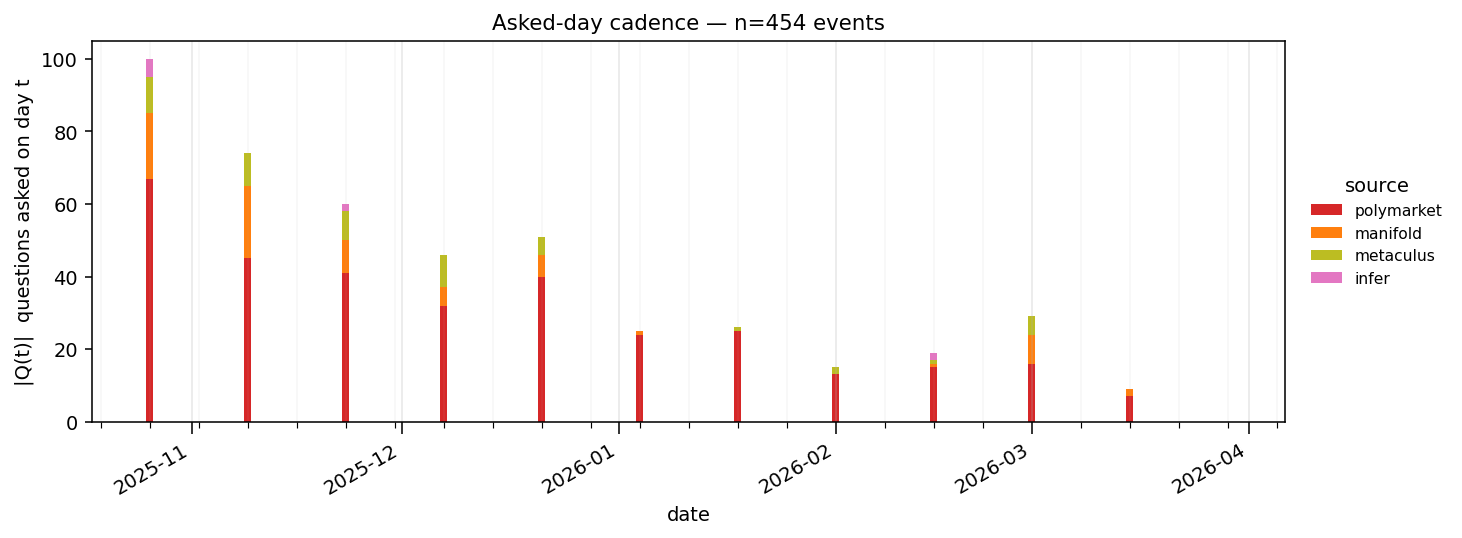
\includegraphics[width=\linewidth]{markets_only_q.png}
  \caption{Asked-day cadence $|Q(t)|$ stacked by source. The pool's
    biweekly Sunday rhythm is visible; the decay over time is the
    censoring effect: questions asked late have more of their resolution
    dates beyond $t_{\max}$ and contribute fewer surviving events.}
  \label{fig:Qt}
\end{figure}

\begin{figure}[h]
  \centering
  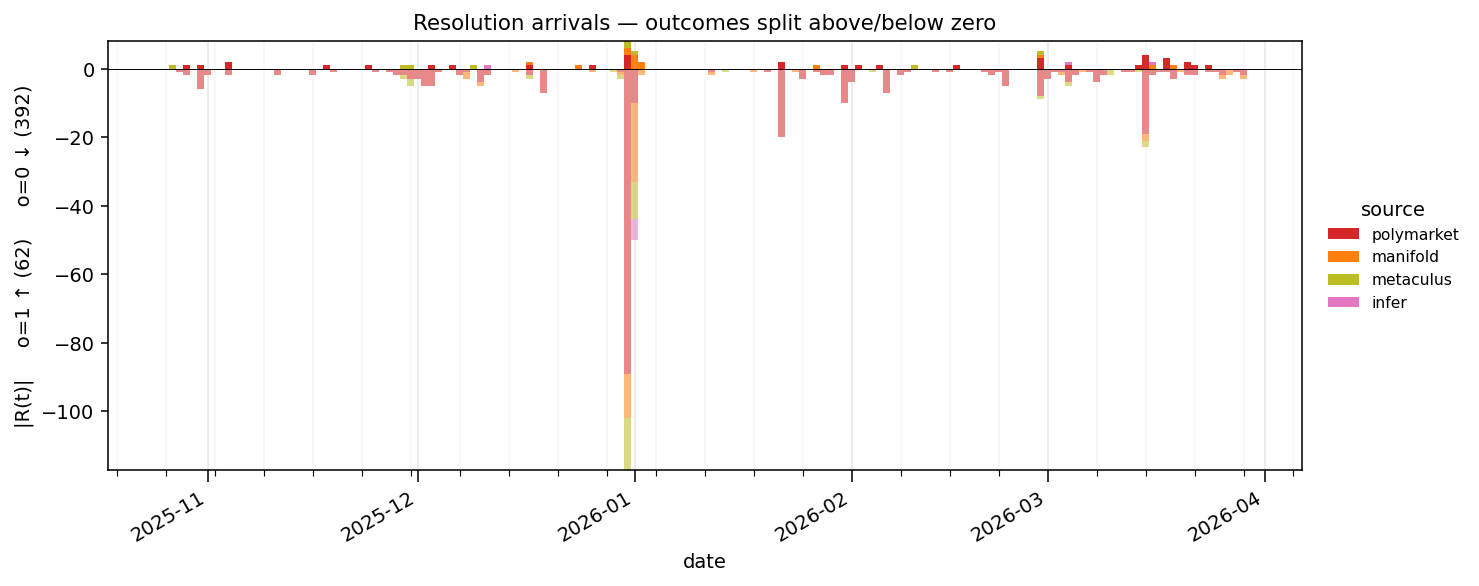
\includegraphics[width=\linewidth]{markets_only_r.png}
  \caption{Resolution arrivals $|R(t)|$. Outcomes split above (\(o = 1\))
    and below (\(o = 0\)) zero so the day-by-day class balance is
    legible. Markets resolve on idiosyncratic dates rather than the
    biweekly grid that governs $Q(t)$.}
  \label{fig:Rt}
\end{figure}

\begin{figure}[h]
  \centering
  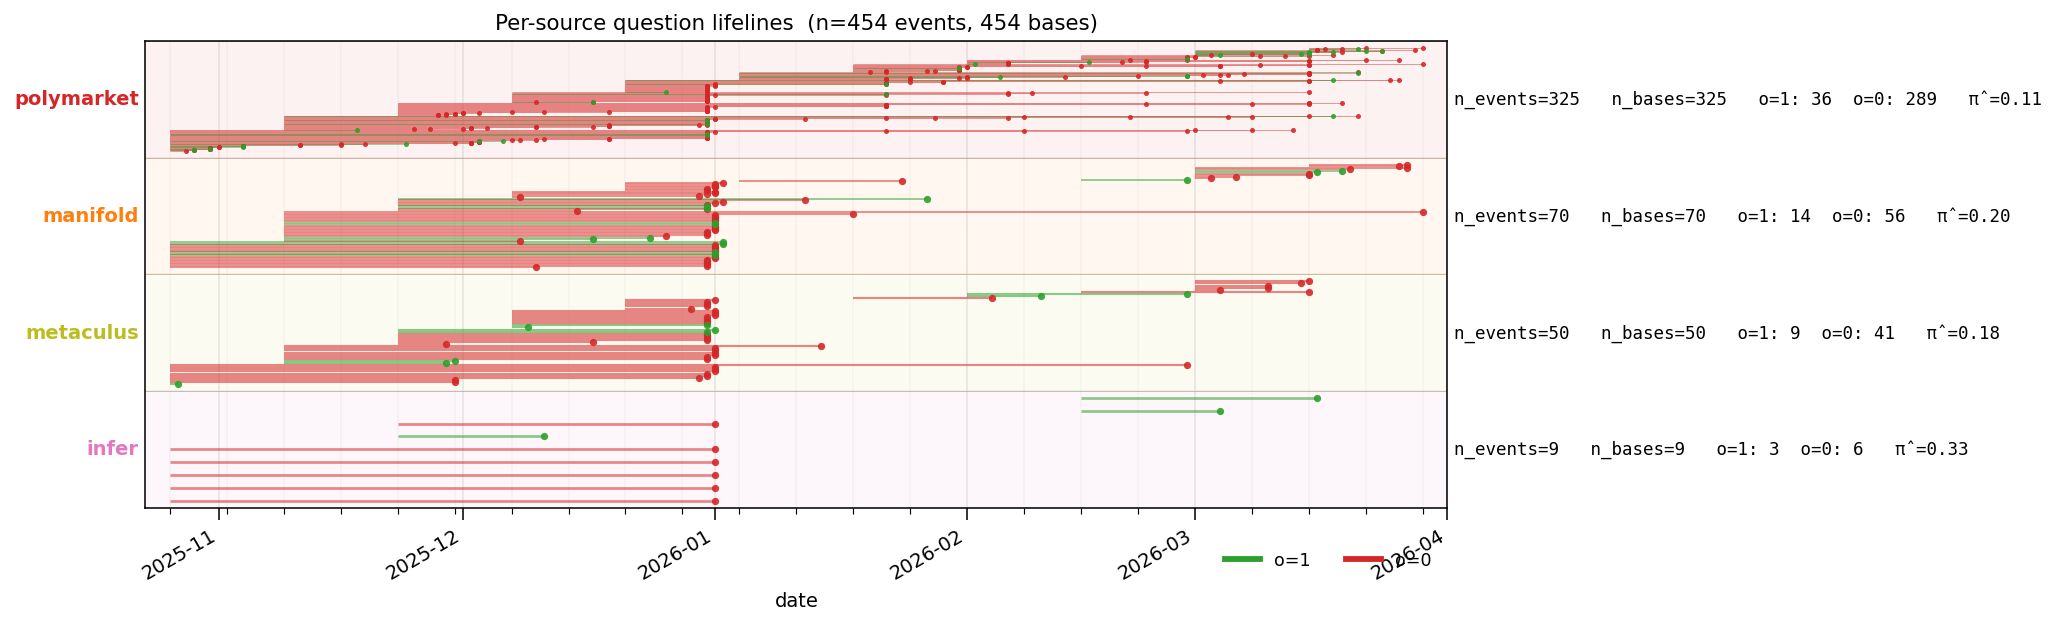
\includegraphics[width=\linewidth]{markets_only_lifelines.png}
  \caption{Per-source question lifelines. Each row is one question,
    sorted by $(f_u, r_u)$; the lifeline runs from $f_u$ to $r_u$ and is
    coloured by outcome (green = 1, red = 0), with an endpoint dot at
    $r_u$. Each source occupies a fixed-height swim lane so rare sources
    (\texttt{infer}, \texttt{metaculus}) are as visible as the
    polymarket-dominated mass. The right-margin labels report
    $n_\text{events}$, $n_\text{bases}$, and $\hat\pi_q$ per source.}
  \label{fig:lifelines}
\end{figure}

\section{Results}
\label{sec:results}

We evaluate five baseline agents on the canonical pool. All LLM agents
use \texttt{gemini-3-flash-preview} via OpenRouter and the Halawi et al.
zero-shot prompt template \cite{halawi2024approaching}. Agents are run in
two regimes:

\begin{description}
  \item[$c = 0$:] no crowd anchor. The market freeze value is hidden
    from the prompt; agents must reason from the question, criteria, and
    background alone. This is the regime that admits algorithmic
    headroom, since the agent cannot ride on a calibrated crowd
    estimate.
  \item[$c = 1$:] the market freeze value is injected into the prompt as
    a freeze field. This is the BLF Table-17 setup. We additionally
    consider a \texttt{+shrink} post-processing layer that performs
    online per-source mixing toward the freeze value.
\end{description}

\paragraph{$c = 0$ headline.}
Figure~\ref{fig:c0} shows the cumulative and rolling-window Brier-index
reward curves over the 454-event run. Two stateless baselines (dashed):
the source-blind running mean (\texttt{empirical}) and zero-shot Flash
(\texttt{flash-zs}); two stateful systems (solid): in-context learning
over past resolutions (\texttt{flash-zs-icl}) and the same with online
Platt calibration on top (\texttt{flash-zs-icl+platt}). The ICL agent
sustains a $\sim$0.05 BI advantage over its stateless counterpart
throughout the run, and the gap is visible from instance $\sim 100$
onward once the memory has accumulated useful examples.

\begin{figure}[h]
  \centering
  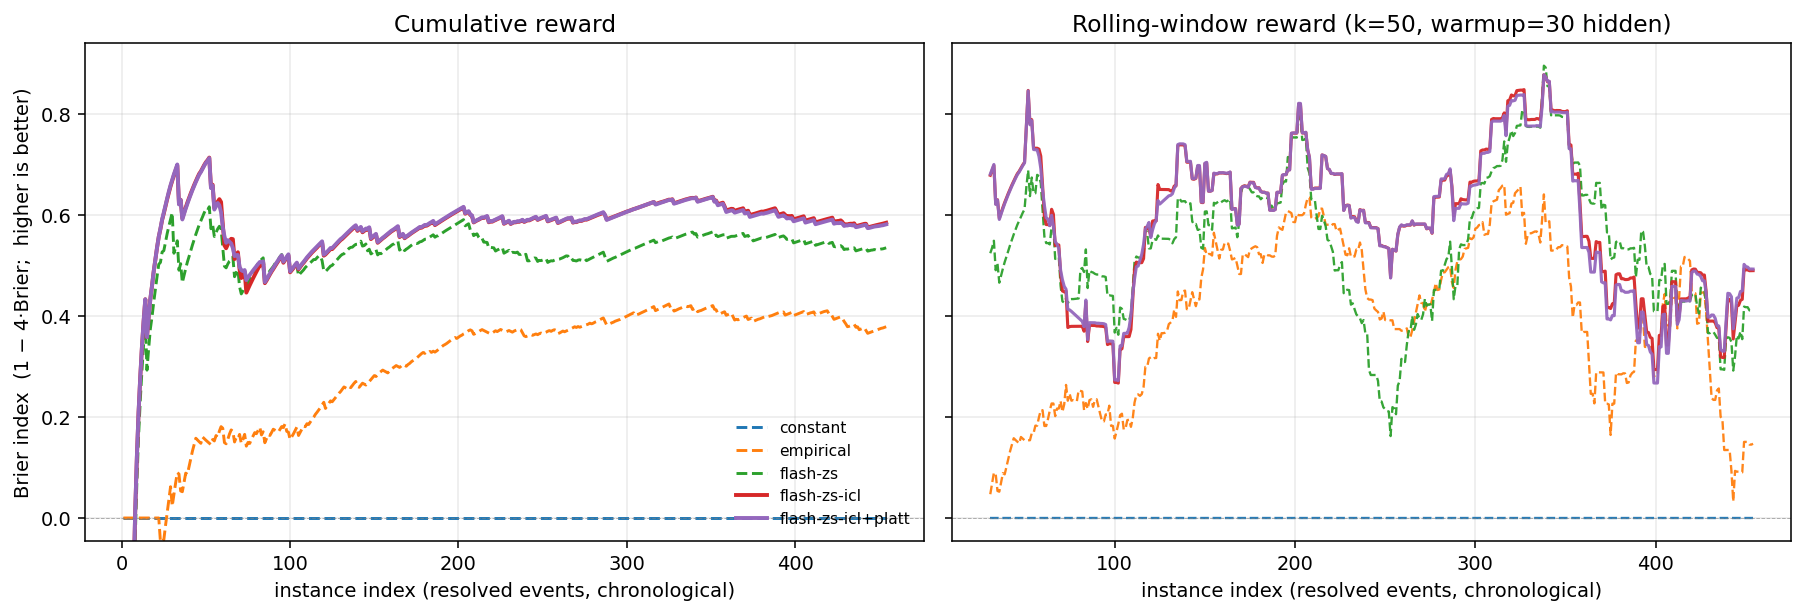
\includegraphics[width=\linewidth]{continual_c0.png}
  \caption{$c = 0$ comparison. Stateless agents (dashed) include the
    empirical running mean and zero-shot Flash; stateful agents (solid)
    add ICL memory and optional online Platt calibration. The
    \texttt{constant} 0.5 baseline anchors $\mathrm{BI} = 0$.
    Left: cumulative Brier index. Right: rolling window $k = 50$ with the
    first 30 events hidden as warmup.}
  \label{fig:c0}
\end{figure}

\paragraph{$c = 1$ appendix.}
Figure~\ref{fig:c1} reports the same comparison with the freeze value
available --- both injected into the prompt and exposed to a
\texttt{+shrink} post-processing layer. The \texttt{market-value}
baseline (just predict $p = $ freeze value) attains
$\mathrm{BI}_{\text{event}} = 0.81$, well above any LLM agent without
shrinkage. The \texttt{+shrink} layer recovers this number by learning
$\alpha \to 0$ for sources where the LLM trails the crowd, effectively
falling back to the freeze value where the LLM cannot improve on it.
The visible result is that all LLM-plus-shrink lines converge to the
crowd baseline; algorithmic differences between agents are
\emph{erased} once a calibrated crowd anchor is available. This is the
motivation for centring CFB on the $c = 0$ regime.

\begin{figure}[h]
  \centering
  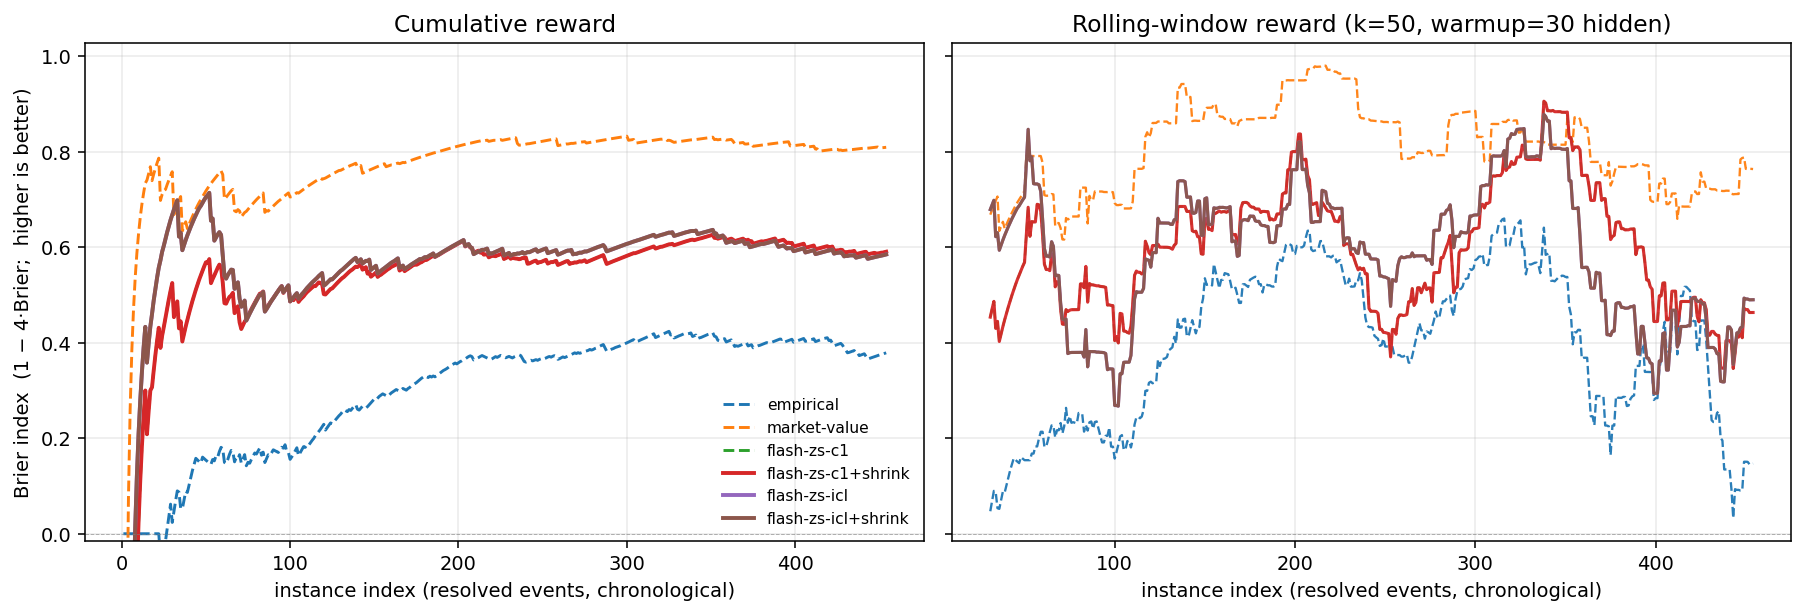
\includegraphics[width=\linewidth]{continual_c1.png}
  \caption{$c = 1$ comparison. The crowd anchor (\texttt{market-value},
    dashed orange) dominates all LLM agents on its own. With the
    \texttt{+shrink} post-layer, every LLM agent converges to within
    a few thousandths of the crowd baseline because the per-source
    online $\alpha$ correctly identifies that the LLM cannot improve on
    the crowd at this volume.}
  \label{fig:c1}
\end{figure}

\paragraph{Final scores.} Table~\ref{tab:scores} reports both
event-weighted and source-weighted Brier indices for every agent on the
canonical pool.

\begin{table}[h]
  \centering
  \begin{tabular}{lrr}
    \toprule
    \textbf{xid} & $\mathrm{BI}_{\text{event}}$ & $\mathrm{BI}_{\text{source}}$ \\
    \midrule
    \multicolumn{3}{l}{\emph{$c = 0$ — no crowd anywhere}} \\
    constant            & 0.000 & 0.000 \\
    empirical           & 0.379 & 0.116 \\
    flash-zs            & 0.535 & 0.270 \\
    flash-zs-icl        & 0.585 & 0.392 \\
    flash-zs-icl+platt  & 0.581 & 0.432 \\
    \midrule
    \multicolumn{3}{l}{\emph{$c = 1$ — freeze value available}} \\
    market-value           & 0.809 & 0.654 \\
    flash-zs-c1            & 0.590 & 0.374 \\
    flash-zs-c1+shrink     & 0.807 & 0.650 \\
    flash-zs-c1+shrink+platt & 0.809 & 0.649 \\
    flash-zs-icl+shrink    & 0.802 & 0.641 \\
    \bottomrule
  \end{tabular}
  \caption{Brier indices on the canonical CFB pool ($N = 454$ events).}
  \label{tab:scores}
\end{table}

\bibliographystyle{plain}
\begin{thebibliography}{1}
\bibitem{halawi2024approaching}
Halawi, D., Zhang, F., Yueh-Han, C., and Steinhardt, J. (2024).
\newblock Approaching Human-Level Forecasting with Language Models.
\newblock \emph{arXiv preprint arXiv:2402.18563}.
\end{thebibliography}

\end{document}
